\documentclass[a4paper]{article}

\usepackage[slovene]{babel}
\usepackage{amsfonts,amssymb,amsmath}
\usepackage[utf8]{inputenc}
\usepackage[T1]{fontenc}
\usepackage{lmodern}

\usepackage{graphicx}

\begin{document}

\title{\Huge\textbf{Projekt pri predmetu Matematično modeliranje}} 
\author{\large\textsc{Tjaša Vrhovnik}\\
	Fakulteta za matematiko in fiziko\\
	Oddelek za matematiko}

\thispagestyle{empty}

\maketitle

\newpage

\tableofcontents

\newpage

%%%%%%%%%%%%%%%%%%%%%%%%%%%%%%%%%%%%%%%%%%%%%%%%%%%%%%%%%%%%%%%%%%%%%%%%%%%%

\section{Naloga}

Rešujemo naslednji problem: V ravnini sta dani dve točki, $T_{1}(x_1,y_1)$ in $T_{2}(x_2,y_2)$, kjer je $y_1 > y_2$ in $x_1 < x_2$. Med vsemi kubičnimi polinomi, ki potekajo skozi točke $T_1$, $T_2$ in $T_3 = T_1 + \frac{1}{2} (T_2-T_1)$, iščemo tistega, ki minimizira čas potovanja kroglice po njegovem grafu od $T_1$ do $T_2$.

\section{Izpeljava}

Naloga se zdi podobna znamenitemu problemu o brahistohroni, ki ga je zastavil Jacob Bernoulli.
Označimo iskan polinom z $r(x) = a_{3}x^3+a_{2}x^2+a_{1}x+a_{0}$. Polinom $r$ bo določen, ko bomo poznali njegove koeficiente $a_{3}$, $a_{2}$, $a_{1}$ in $a_{0}$.
Za lažje računanje za začetek prestavimo točke tako, da bo $T_1$ v koordinatnem izhodišču. Označimo nove točke:
\begin{align*}
T_{1}' &= (0,0), \\
T_{2}' &= T_2 - T_1 = (x_2-x_1, y_2-y_1), \\
T_{3}' &= T_3 - T_1 = \frac{1}{2}(T_2 - T_1) = \frac{1}{2}T_{2}'.
\end{align*}
S tem bo graf transliranega polinoma $p(x) = ax^3+bx^2+cx+d$ med $T_{1}'$ in $T_{2}'$ ves čas pod abscisno osjo. Če bi graf dosegel nenegativno vrednost med točkama $T_{1}'$ in $T_{3}'$, bi bil vodilni koeficient polinoma $p$ pozitiven. To bi pomenilo, da bi se kroglica iz začetne točke dvigala, kar fizikalno ni mogoče. Predvidevamo tudi, da so vrednosti polinoma med točkama $T_{3}'$ in $T_{2}'$ povsod negativne; to bomo kasneje potrdili z numeričnimi primeri.

Izračunajmo koeficiente polinoma $p$. Vemo, da je kubični polinom enolično določen s štirimi točkami v ravnini. V našem primeru so znane tri točke na polinomu, kar pomeni, da bomo imeli en prost parameter. Vstavimo koordinate točk $T_{1}'$, $T_{2}'$ in $T_{3}'$ v izraz za polinom $p$ in računajmo:
\begin{equation}
\label{Eq:p(T_{1}')}
p(0) = d = 0,
\end{equation}
%
\begin{equation}
\label{Eq:p(T_{2}')}
p(x_2-x_1) = a(x_2-x_1)^3+b(x_2-x_1)^2+c(x_2-x_1) = y_2-y_1,
\end{equation}
%
\begin{equation}
\label{Eq:p(T_{3}')}
p \left(\frac{x_2-x_1}{2} \right) = a \left(\frac{x_2-x_1}{2} \right)^3+b \left(\frac{x_2-x_1}{2} \right)^2+c \frac{x_2-x_1}{2} = \frac{y_2-y_1}{2}.
\end{equation}
%
Pomnožimo enačbo~\eqref{Eq:p(T_{3}')} z $2$ in jo odštejmo od enačbe~\eqref{Eq:p(T_{2}')}. Dobimo
\begin{align}
\frac{3}{4} a(x_2-x_1)^3 + \frac{1}{2} b(x_2-x_1)^2 &= 0, \nonumber \\
\frac{3}{2} a(x_2-x_1) + b &= 0, \nonumber \\
b &= -\frac{3}{2} a(x_2-x_1).
\end{align}
%
Koeficient $c$ izračunamo iz enačbe~\eqref{Eq:p(T_{2}')}, pri čemer upoštevamo zgornji izraz za $b$. Računamo
\begin{align}
c(x_2-x_1) &= y_2 - y_1 - a(x_2-x_1)^3 - b(x_2-x_1)^2 \nonumber \\
 &= y_2 - y_1 - a(x_2-x_1)^3 + \frac{3}{2} a(x_2-x_1)^3 \nonumber \\
 &= y_2 - y_1 + \frac{1}{2} a(x_2-x_1)^3, \nonumber \\
c &= \frac{y_2-y_1}{x_2-x_1} + \frac{1}{2} a(x_2-x_1)^2.
\end{align}
%
Koeficienti polinoma $p$ se izražajo s parametrom $a$, katerega ne poznamo. Polinom $p$ je torej funkcija dveh spremenljivk, $p = p(x,a)$. Spremenljvko $a$ bomo določili z minimizacijo časa potovanja po grafu polinoma.

Čas, ki ga kroglica potrebuje za pot med točkama $T_{1}'$ in $T_{2}'$ se izraža z integralom 
\begin{equation}
\label{Eq:Cas}
t = \int_{T_{1}'}^{T_{2}'} \frac{ds}{v}.
\end{equation}
%
Upoštevajmo zakon o ohranitvi energije, ki v našem primeru pravi, da se vsota kinetične in potencialne energije kroglice med potovanjem ohranja. Uporabimo razmislek, da je graf polinoma ves čas pod abscisno osjo -- enačba se tako glasi
\begin{equation*}
\frac{1}{2}mv^2 = mg(-p),
\end{equation*}
od koder izrazimo hitrost potovanja kroglice
\begin{equation*}
v = \sqrt{2g(-p)}.
\end{equation*}
%
Vemo še, da je ločna dolžina enaka $ds^2 = dx^2 + dp^2$. Označimo parcialni odvod polinoma $p$ po spremenljivki $x$ s $p'=\frac{dp}{dx}$. Enačba~\eqref{Eq:Cas} tako dobi obliko
\begin{equation}
\label{Eq:CasInt}
T(a) = \int_{0}^{x_2-x_1} \sqrt{ \frac{1+p'^2}{-2gp}} dx,
\end{equation}
kjer smo s $T$ označili funkcijo časa, odvisno od spremenljivke $a$. Naša naloga je poiskati njen minimum.
Analitično iskanje minimuma funkcije $T$ je zahtevno; pomagali si bomo z numeriko in s pomočjo programa Matlab poiskali vrednost $a$, ki ustreza minimalni vrednosti funkcije $T$.

%%%%%%%%%%%%%%%%%%%%%%%%%%%%%%%%%%%%%%%%%%%%%%%%%%%%%%%%%%%%%%%%%%%%%%%%%%%%% Numerična rešitev
\section{Numerična rešitev}

Vrednost spremenljivke $a$, ki minimizira funkcijo časa $T$ poiščemo numerično. 

%%%
\subsection{Program \texttt{doloci\_polinom.m}}

Oglejmo si program \texttt{doloci\_polinom.m} v Matlabu.
Program kot argumente sprejme koordinate točk $T_1$ in $T_2$ pri čemer velja $x_1, y_1, x_2, y_2 \in \mathbb{R}$, $y_1 > y_2$ in $x_1 < x_2$. Kot smo razmislili v prejšnjem poglavju, je smiselno točke translirati tako, da točka $T_1$ leži v koordinatnem izhodišču. Koeficiente transliranega polinoma $p$ definiramo kot funkcije spremenljivke $a$, ter definiramo polinom in njegov odvod, ki sta funkciji spremenljivk $a$ in $x$. Funkcijo $T$ definiramo kot v enačbi~\eqref{Eq:CasInt}. Za minimizacijo te funkcije uporabimo vgrajeno funkcijo \texttt{fminsearch}, ki vrne iskano vrednost spremenljivke $a$, pri kateri je čas potovanja kroglice po grafu polinoma najmanjši. Vrednost v programu označimo z $A$.
Kako smo določili začetni približek za vrednost $A$, ki je obvezen argument funkcije \texttt{fminsearch}? Že v začetku smo premislili, da bo vodilni koeficient polinoma negativen. Če izberemo $a=0$, se translirani polinom glasi $p(x) = \frac{y_2-y_1}{x_2-x_1} x$, kar je premica skozi točke $T_{1}'$, $T_{2}'$ in $T_{3}'$. Z naraščanjem absolutne vrednosti $a$ postaja graf polinoma čedalje bolj ukrivljen. Tako za $a<0$ kmalu doseže nenegativne vrednosti med točkama $T_{3}'$ in $T_{2}'$; izračunan čas je v tem primeru kompleksno število, zato smo v težavah. Vendar na konkretnih primerih ugotovimo, da je za negativne vrednosti $a$, ki so blizu $0$ potreben čas manjši od časa potovanja po premici, z manjšanjem $a$ od neke vrednosti $a$ dalje pa se čas povečuje. Nadalje obstaja še manjša vrednost $a$, pri kateri graf polinoma preide abscisno os. Od tod sklepamo, da je ustrezen začetni približek $A=0$.

Program \texttt{doloci\_polinom.m} vrne vodilni koeficient polinoma $p$ skozi translirane točke, od koder lahko izračunamo ostale koeficiente polinoma. 
Našli smo torej polinom, ki minimizira čas potovanja kroglice skozi točke $T_{1}'$, $T_{2}'$ in $T_{3}'$. Vendar je naša naloga poiskati polinom $r$, ki vsebuje točke $T_1$, $T_2$ in $T_3$. Časa potovanj po grafih obeh polinomov sta enaka, saj se obliki (ukrivljenosti) polinomov ujemata. Iskani polinom namreč dobimo tako, da polinom skozi premaknjene točke transliramo za krajevni vektor točke $T_1$.
Polinom skozi prvotne točke, ki nas zanima, ustreza zvezi
\begin{align}
\label{Eq:r(x)}
r(x) = a(x-x_1)^3 + b(x-x_1)^2 + c(x-x_1) + d + y_1.
\end{align}
Ker poznamo koeficiente $a$, $b$, $c$ in $d$, vrednosti $x_1$ in $y_1$ pa sta koordinati točke $T_1$, poznamo tudi iskani polinom $p$.

%%%
\subsection{Program \texttt{risi\_polinom.m}}

Za vizualizacijo uporabimo program \texttt{risi\_polinom.m}.
Ta najprej odpre koordinatno mrežo velikosti $[0,1] \times [0,1]$, na kateri uporabnik s klikom izbere dve točki. Zaradi lažje predstave program koordinate izbranih točk pomnoži s faktorjem $10$, tako dobljeni točki pa ustrezata točkama $T_1$ in $T_2$, ki določata polinom.
Ko sta točki izbrani, program s pomočjo klica programa \texttt{doloci\_polinom.m} izračuna koeficient $a$, od tod pa še koeficiente $b$, $c$ in $d$ transliranega polinoma skozi koordinatno izhodišče. Kot v enakosti~\eqref{Eq:r(x)} definira še iskani polinom $r$ skozi točke $T_1$, $T_2$ in $T_3$.

Izrišeta se dve sliki.
Na prvi je s črtkano črto predstavljen transliran polinom $p$, ki poteka skozi koordinatno izhodišče, in na njem označene točke $T_{1}'$, $T_{2}'$ in $T_{3}'$.
Polna črta predstavlja iskani polinom $r$, oznake $\times$ pa so izbrane točke $T_1$, $T_2$ in $T_3$, ki ga določajo.  
%
Vemo, da je najhitrejša pot kroglice po grafu med dvema točkama v ravnini, ki ustrezata $y_1 > y_2$ in $x_1 < x_2$, brahistohrona. Zato bomo naredili primerjavo brahistohrone s kubičnim polinomom, ki imata skupni začetno in končno točko $T_1$ in $T_2$, polinom pa vsebuje še točko $T_3 = T_1 + \frac{1}{2} (T_2-T_1) $.
Druga slika predstavlja brahistohrono in kubični polinom, ki minimizira čas potovanja skozi dane točke. S simbolom $\times$ so označene točke $T_1$, $T_2$ in $T_3$.

Program izračuna in izpiše še čas potovanja po kubičnem polinomu, brahistohroni in premici skozi dane točke.
Programi, ki določijo, narišejo brahistohrono in izračunajo čas potovanja po brahistohroni ter premici (\texttt{isci\_theta.m}, \texttt{risi\_brahi.m} in \texttt{cas\_brahi.m}) so bili napisani na vajah predmeta Matematično modeliranje. 

%%%%%%%%%%%%%%%%%%%%%%%%%%%%%%%%%%%%%%%%%%%%%%%%%%%%%%%%%%%%%%%%%%%%%%%%%%%%% Primeri
\section{Primeri}
%%%%%%%%%%%%%%%%%%%%%%%
\subsection{Vzorčni primer}

Najprej si oglejmo vzorčni primer, kjer so koordinate točk $T_1$ in $T_2$ naravna števila. Izberimo
\begin{align*}
T_1(1,5), \\
T_2(7,2).
\end{align*}
%
Točke vstavimo v program \texttt{doloci\_polinom.m} in izračunajmo koeficiente polinoma $p$, katerega graf poteka skozi koordinatno izhodišče. Dobimo vrednosti
\begin{align*}
a &= -0.0440, \\
b &= 0.3960, \\
c &= -1.2920, \\
d &= 0.
\end{align*}
%
Če jih vstavimo v enakost~\eqref{Eq:r(x)} in upoštevamo koordinate izbranih točk, dobimo eksplicitno formulo za polinom $r$, ki minimizira čas potovanja skozi izbrane točke $T_1(1,5)$, $T_2(7,2)$ in $T_3(4,3.5)$.

Koordinate točk vstavimo še v program \texttt{risi\_polinom.m} in si oglejmo sliko, ki prikazuje grafa transliranega polinoma skozi koordinatno izhodišče s črtkano črto ter iskanega polinoma z modro barvo.
\begin{figure}[h!]
\begin{center}
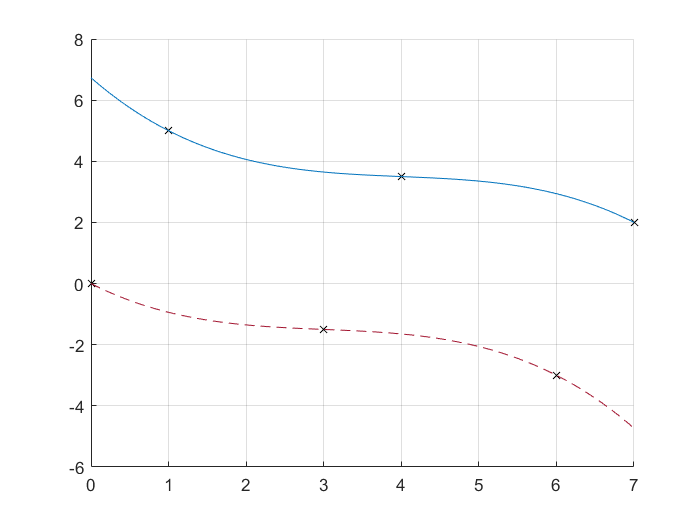
\includegraphics[scale=0.52]{primer2-polinom.png}
\caption{Grafa polinomov, določenih s točkama $T_1(1,5)$ in $T_2(7,2)$.}
\end{center}
\end{figure}
%
S slike vidimo, da graf transliranega polinoma med točkama $T_{1}'$ in $T_{2}'$ v celoti leži pod abscisno osjo, kar je bil eden izmed naših kriterijev.

Opazujmo še vodilni koeficient $a$. Vrednost, ki jo vrne program, znaša $a = -0.0440$. Preden sem definirala funkcije, ki določijo optimalno pot kroglice, sem za občutek narisala nekaj grafov kubičnih polinomov skozi zgoraj izbrane točke in izračunala čas potovanja po njih. S poskušanjem in ugotovitvah, ki so opisana v razdelku o numerični rešitvi, sem prišla do približka $a = -0.05$, kar se zdi dober približek za iskano vrednost v konkretnem primeru. 

Druga slika, ki jo vrne program \texttt{risi\_polinom.m} predstavlja graf iskanega kubičnega polinoma ter brahistohrono. Krivulji imata skupni začetno in končno točko. 
%
\begin{figure}[h!]
\begin{center}
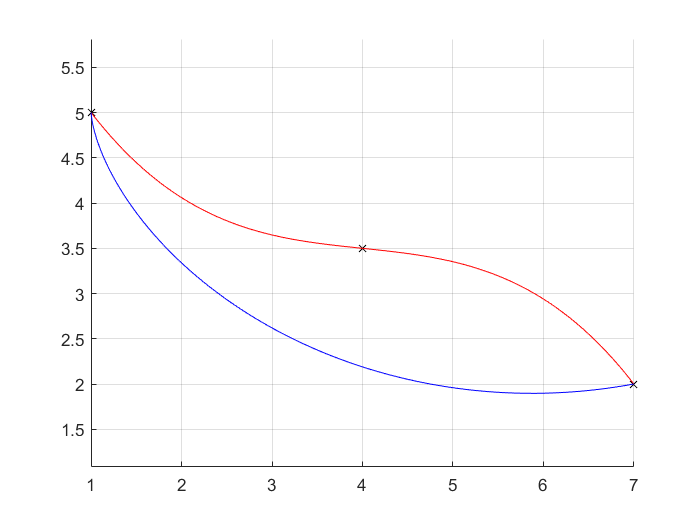
\includegraphics[scale=0.6]{primer2-PolBrah.png}
\caption{Kubični polinom in brahstohrona, določeni s točkama $T_1(1,5)$ in $T_2(7,2)$.}
\end{center}
\end{figure}
%

Spodnje vrednosti so izračunani časi potovanja kroglice po treh krivuljah. Čas potovanja po brahistohroni je res najmanjši, najdlje pa kroglica potrebuje za pot po premici.
%
\begin{align*}
t_{polinom} &= 1.590217900171090, \\
t_{brahistohrona} &= 1.395989176219715, \\
t_{premica} &= 1.749635530559413.
\end{align*}

%%%%%%%%%%%%%%%%%%%%%%%%
\subsection{Primer z uporabo grafičnega vmesnika}

Oglejmo si primer, kjer smo v programu \texttt{risi\_polinom.m} točki $T_1(x_1,y_1)$ in $T_2(x_2,y_2)$ izbrali z grafičnim vmesnikom. Koordinate točk ustrezajo vrednostim
\begin{align*}
x_1 &= 0.930018416206262, \\
y_1 &= 8.983644859813083, \\
x_2 &= 9.456721915285449, \\
y_2 &= 2.792056074766355.
\end{align*}
%
Program izriše naslednji sliki.

\begin{figure}[h!]
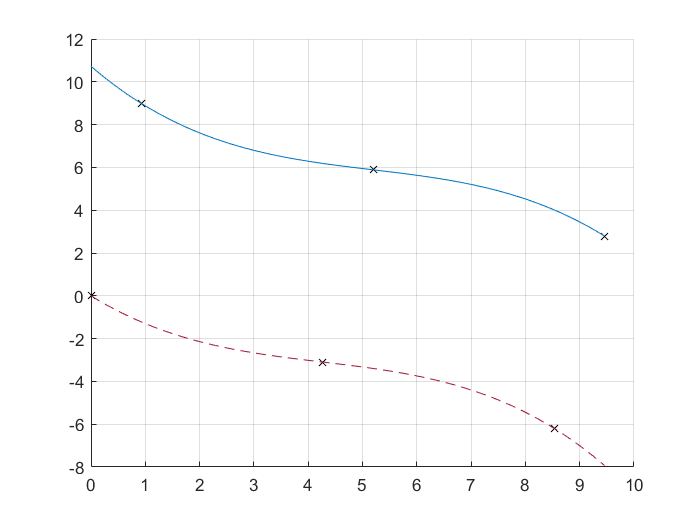
\includegraphics[scale=0.6]{primer1-polinom.png}
\caption{Kubični polinom, ki minimizira čas potovanja kroglice skozi točke $T_1$, $T_2$ in $T_3$, je predstavljen s polno črto. S črtkano črto je predstavljen transliran polinom skozi koordinatno izhodišče.}
\end{figure}

\begin{figure}[h!]
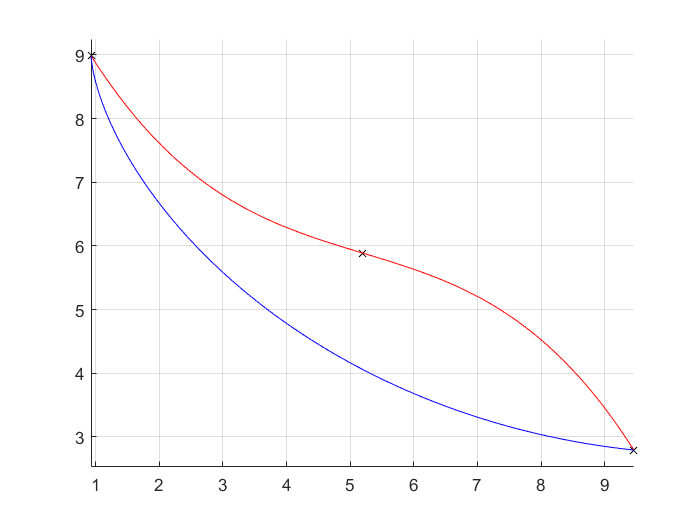
\includegraphics[scale=0.6]{primer1-PolBrah.png}
\caption{Z rdečo barvo je predstavljen kubični polinom, ki minimizira čas potovanja kroglice skozi točke $T_1$, $T_2$ in $T_3$, z modro pa brahistohorna skozi točki $T_1$ in $T_2$.}
\end{figure}

Izračunani časi potovanja po kubičnem polinomu, brahistohorni in premici:
\begin{align*}
t_{polinom} &= 1.800452978985828, \\
t_{brahistohrona} &= 1.657073117759419, \\
t_{premica} &= 1.913116876467396.
\end{align*}
%
Opazimo, da se numerični rezultati ujemajo s pričakovanji: čas potovanja po brahistohroni je najmanjši, sledi mu kubični polinom, premica pa da najpočasnejšo pot.

Izračunajmo še vrednost koeficientov polinoma $p$:
\begin{align*}
a &= -0.023312500000000, \\
b &= 0.269188535911602, \\ 
c &= -1.507190104569076, \\ 
d &= 0.
\end{align*}
Če koeficiente vstavimo v zvezo~\eqref{Eq:r(x)} in upoštevamo koordinate izbranih točk $T_1$ in $T_2$, dobimo eksplicitno formulo iskanega polinoma $r$.

%%%%%%%%%%%%%%%%%%%%%%%%%%%%%%%%%%%%%%%%%%%%%%%%%%%%%%%%%%%%%%%%%%%%%%%%%%%%
% Literatura

\begin{thebibliography}{99}

\bibitem{zapiski} Zapiski s predavanj prof.~E.~Žagarja pri predmetu Matematično modeliranje, Univerza v Ljubljani, Fakulteta za matematiko in fiziko (študijsko leto 2018/2019).

\end{thebibliography}

\end{document}